\begin{figure}[H]
\centering
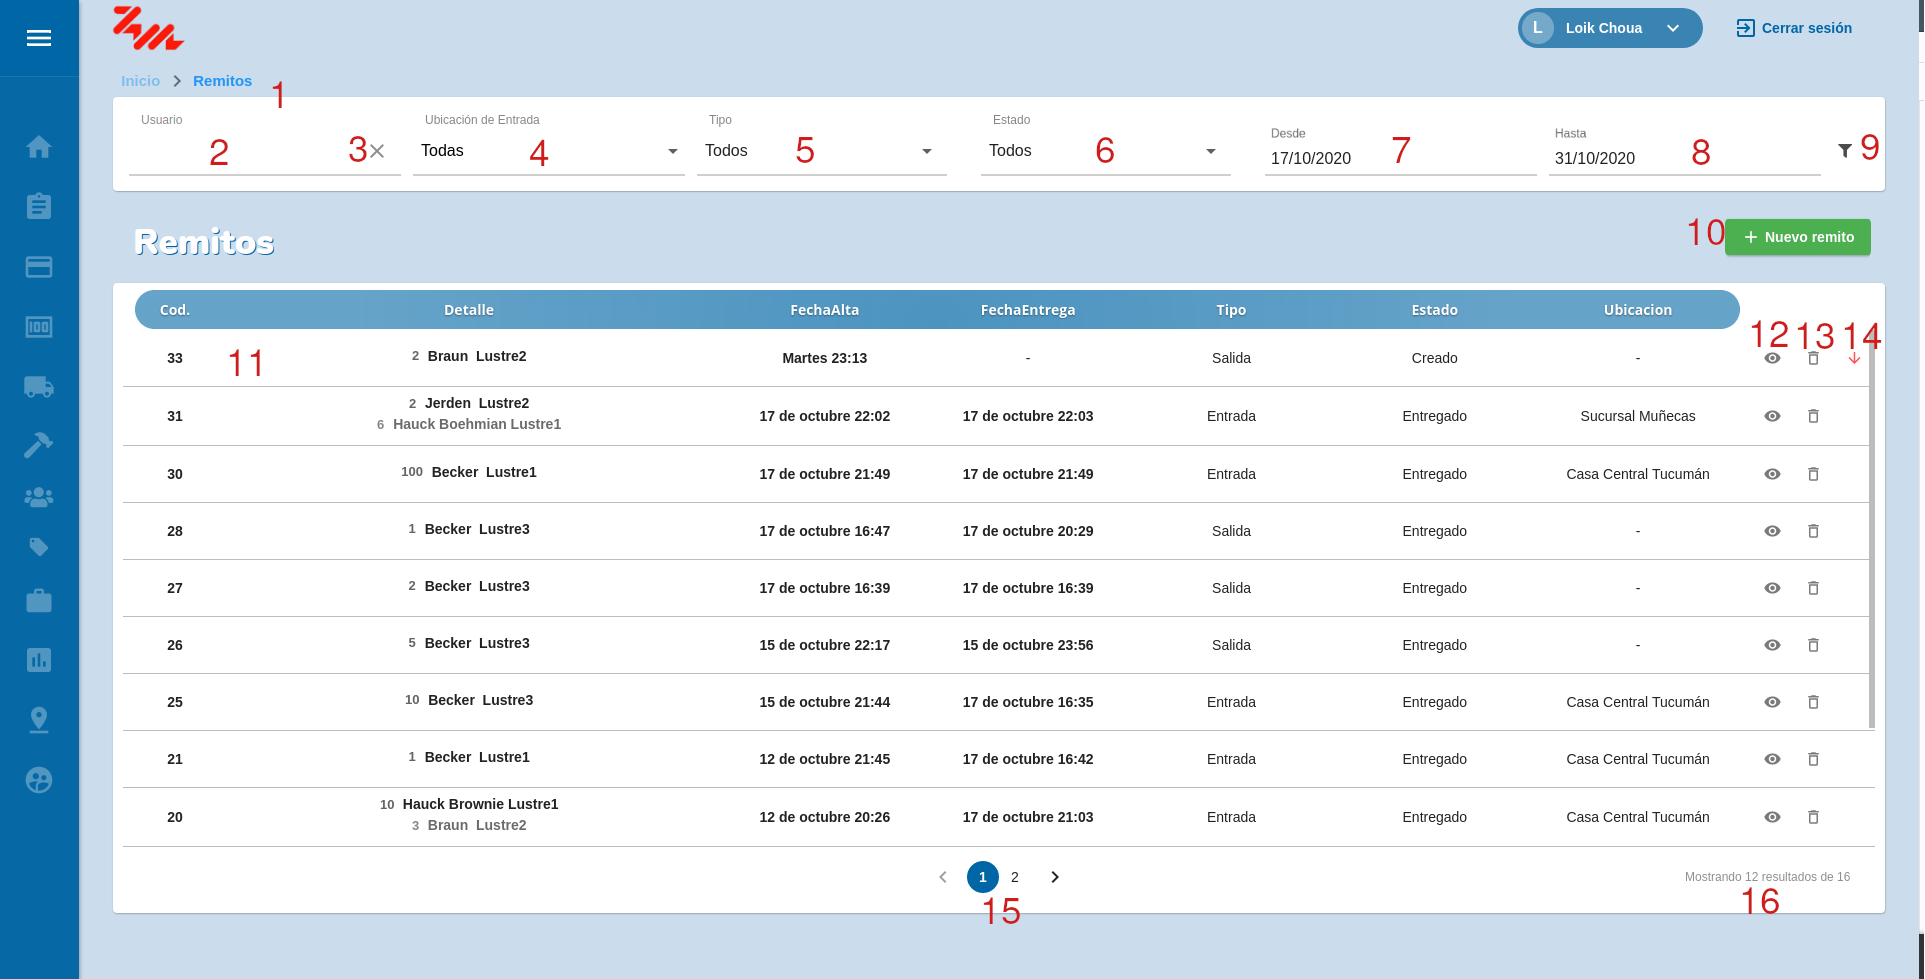
\includegraphics[width=\textwidth,height=\textheight,keepaspectratio]{Escenarios/AD-16-00}
\caption{Escenario - AD-16-00}
\label{fig:AD-16-00}
\end{figure}
Este escenario muestra toda la información referida a los remitos, junto con las acciones disponibles.
El botón \textbf{AD-16-01} permite navegar al escenario. El campo \textbf{AD-16-02} permite al usuario buscar remitos de acuerdo al empleado que la realizó el campo cuenta con el botón \textbf{AD-16-03} que permite borrar el texto ingresado en el campo. La lista desplegable \textbf{AD-16-04} permite filtrar de acuerdo a la ubicación de entrada de los remitos. La lista desplegable \textbf{AD-16-5} permite filtrar de acuerdo al tipo de remito. La lista desplegable \textbf{AD-16-06} permite al usuario filtrar por los estados en los cuales puede encontrarse el remito.  Los campos \textbf{AD-16-07} y \textbf{AD-16-08} permiten al usuario filtrar los ventas de acuerdo a un rango de fechas en el cual fueron creados. El botón \textbf{AD-16-09} permite visualizar más filtros de búsqueda disponibles, como ser el producto, la tela y el lustre.
El botón \textbf{AD-16-10} permite al usuario crear un nuevo remito y navega al escenario \textbf{AD-17-00}.
El campo \textbf{AD-16-11} muestra la información relacionada a los remitos especificando el código, el detalle de remito, la fecha de creación, la fecha de entrega, el tipo de remito, el estado en el cúal se encuentra y la ubicación de entrada en caso de existir. El botón \textbf{AD-16-12} permite navegar al escenario \textbf{AD-19-00} para ver el remito, el botón \textbf{AD-16-13} permite al usuario borrar el remito y el botón \textbf{AD-16-14} permite al usuario dar de baja un remito en caso de poder realizar la acción.. 
En \textbf{AD-16-15} se mostrarán las páginas de resultado, pudiendo cambiar de página. En \textbf{AD-16-16} se mostrará cuantos resultados se están visualizando y el total.
\\
